\chapter{Tensores}
\section{Tensores Cartesianos}

En muchas 'areas de la F'isica es 'util, y frecuentemente necesario, definir \textit{objetos con m'ultiples componentes} respecto a un sistema de coordenadas (SC). En general, los valores de las componentes de estos objetos cambian al ser calculados respecto de otro SC. En particular, es posible \textit{clasificar} este tipo de objetos de acuerdo a c'omo cambian sus componentes bajo una transformaci'on de coordenadas (TC). Esta clasificaci'on permite en particular definir \textbf{tensores} como conjunto de cantidades (las ``componentes del tensor") tales que su relaci'on al cambiar de SC es sencilla (en particular, lineal y homog'enea). En este tipo de an'alisis es importante recordar que \textit{la definici'on de vectores y tensores depende del tipo de transformaci'on} (en general, de coordenadas) bajo consideraci'on. Esto se debe a que, \textit{algunas cantidades pueden formar tensores respecto a un tipo de transformaci'on, pero no serlo respecto a otro tipo de transformaciones}. En otras palabras, la definici'on de tensores es relativa a la transformaci'on considerada. En distintos contextos y teor'ias f'isicas es conveniente considerar transformaciones de distinto tipo (que en general est'an relacionadas con la invariancia de las leyes f'isicas respectivas bajo ese tipo de transformaci'on). Por ejemplo, en mec'anica de Newton (y en general, en teor'ias no-relativistas) es conveniente asegurar que las leyes f'isicas consideradas sean v'alidas independientemente de la orientaci'on de los ejes cartesianos elegidos para un determinado c'alculo. En otras palabras, es necesario considerar c'omo cambian las diversas cantidades bajo \textbf{rotaciones}. Para esto, es 'util definir cantidades que sean vectores y tensores respecto a transformaciones ortogonales de coordenadas (TOC, es decir, rotaciones). Por otro lado, en la teor'ia de Relatividad Especial se considera que $(ct,x,y,z)$ son las cuatro coordenadas asociadas a un evento dado, respecto a un Sistema de Referencia Inercial (SRI). Las transformaciones de las coordenadas del mismo evento entre dos SRI's son en ese caso las \textbf{transformaciones de Lorentz}, que pueden expresarse como una transformaci'on lineal de las coordenadas $(ct,x,y,z)$. En este contexto es 'util entonces considerar (definir) cantidades que transformen como ``cuadri"-tensores bajo transformaciones de Lorentz. Note, sin embargo, que un vector respecto a TOC no define necesariamente un vector bajo transformaciones de Lorentz. 

Analizaremos primero la definici'on, las propiedades b'asicas y la utilidad pr'actica de los tensores respecto a TOC.

\section{Bases ortogonales}

Considere un espacio Euclideano $n$-dimensional ($E_n$), donde cada punto de $E_n$ tiene coordenadas $x_i$, $i=1,\cdots, n$, con respecto a un \textbf{sistema ortogonal de coordenadas} (SOC) $K$. 

Consideramos una \textbf{base ortonormal} (BON) $\lbrace\hat{e}_i\rbrace$ ($i=1,\cdots, n$) de vectores, es decir, tal que
\begin{equation}
\boxed{\hat{e}_i\cdot \hat{e}_j=\delta_{ij},}
\end{equation}
donde $\delta_{ij}$ denota la \textbf{Delta de Kronecker}, definida como los $n^2$ valores dados por
\begin{equation} \label{DK}
\delta_{ij}:=\begin{cases} 1, & \text{si } i=j \\ 0, & \text{si } i\neq j\end{cases} .
\end{equation}
Note que esta Delta de Kronecker puede ser representada matricialmente por la matriz identidad $n\times n$. 

En el espacio euclideano $E_n$ es posible definir (consistentemente) el \textbf{vector posici'on} $\vec{x}$, que une el origen del SCO con un punto con coordenadas $x_i$, por
\begin{equation}
\vec{x}=\sum_{i=1}^n x_i\hat{e}_i.
\end{equation}
En este sentido, las coordenadas $x_i$ son componentes del vector $\vec{x}$ en la base $\lbrace\hat{e}_i\rbrace$, y pueden expresarse como
\begin{equation}\label{x2}
x_i=\vec{x}\cdot\hat{e}_i.
\end{equation}

En general, la BON $\lbrace\hat{e}_i\rbrace$ permite descomponer cada vector $\vec{A}$ en sus respectivas componentes:
\begin{equation}\label{V1}
\vec{V}=\sum_{i=1}^nv_i\hat{e}_i,
\end{equation}
donde
\begin{equation}\label{v2}
v_i=\vec{V}\cdot\hat{e}_i.
\end{equation}


\section{Transformaciones ortogonales}
\begin{figure}[H]
\centering
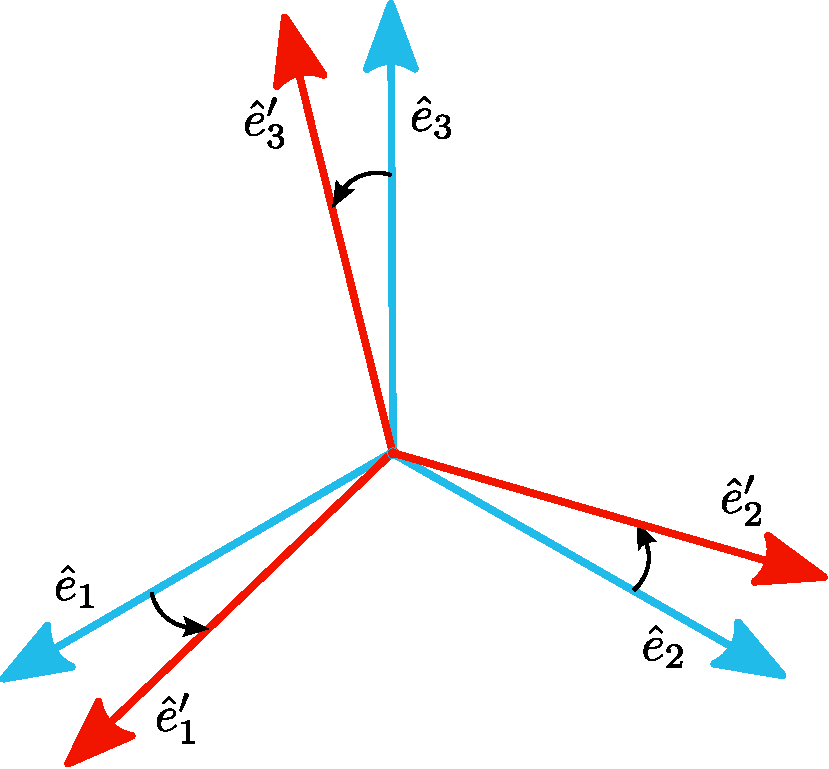
\includegraphics[angle=0,width=0.3\textwidth]{figs/fig-rotacion-bases.pdf}
\caption{Una transformaci'on ortogonal (rotaci'on) de bases ortonormales.}
\label{fig-rotacion}
\end{figure}
Consideremos ahora un nuevo SOC $x'_i$ relacionado con el SOC $x_i$ por medio de una \textbf{transformaci'on ortogonal (TO) de coordenadas}, es decir, una \textbf{rotaci'on}, ver figura \ref{fig-rotacion}.


Esta transformaci'on induce una nueva BON $\lbrace\hat{e}'_i\rbrace$. Respecto a esta nueva base, un vector $\vec{V}$ tiene componentes $\vec{v}_i$ tales que
\begin{equation}\label{V2}
\vec{V}=\sum_{i=1}^nv'_i\hat{e}'_i.
\end{equation}

Es posible relacionar las bases $\lbrace\hat{e}_i\rbrace$  y $\lbrace\hat{e}'_i\rbrace$ ya que cada vector $\hat{e}'_i$ puede escribirse como una combinaci'on lineal de los vectores base $\hat{e}_i$, esto es, existe una relaci'on de la forma
\begin{equation}\label{epe0}
\hat{e}'_i=\sum_{j=1}^n a_{ij}\hat{e}_j.
\end{equation}

La condici'on que la transformaci'on \eqref{epe0} sea efectivamente una TO, es decir, que transforme una BON en una nueva BON impone ($n(n+1)/2$) condiciones sobres los ($n^2$) coeficientes (la ``matriz'') de transformaci'on $a_{ij}$. En efecto,
\begin{align}
\delta_{ij} &= \hat{e}'_i\cdot \hat{e}'_j \\
&= \left(\sum_{k=1}^na_{ik}\hat{e}_k\right)\cdot \left(\sum_{l=1}^na_{jl}\hat{e}_l\right) \\
&=\sum_{k=1}^n\sum_{l=1}^n a_{ik}a_{jl}\left(\hat{e}_k\cdot \hat{e}_l\right) \\
&= \sum_{k=1}^n\sum_{l=1}^na_{ik}a_{jl}\,\delta_{kl} \\
&= \sum_{k=1}^na_{ik}a_{jk}, 
\end{align}
y por lo tanto,
\begin{equation}\label{aad1}
\boxed{\sum_{k=1}^n a_{ik}a_{jk}=\delta_{ij}.}
\end{equation}
En \textbf{notaci'on matricial}, 
\begin{equation} \label{aat1}
\mathbb{A}\cdot(\mathbb{A}^\top)=\mathbb{I}.
\end{equation}
Al calcular el determinante de (\ref{aat1}) encontramos que
\begin{equation}
(\det\mathbb{A})^2=1,
\end{equation}
por lo que necesariamente $\det\mathbb{A}=1$ o bien $\det\mathbb{A}=-1$. Si $\det\mathbb{A}=1$ decimos que la TO es una \textbf{transformaci'on propia}, mientras que si $\det\mathbb{A}=-1$ ella es \textbf{impropia}. En todo caso $\det\mathbb{A}\neq 0$, de modo que la inversa $\mathbb{A}^{-1}$ siempre existe y es 'unica. De  (\ref{aat1}) vemos entonces que la matriz inversa de una transformaci'on ortogonal coincide con su transpuesta,
\begin{equation}\label{corto}
\mathbb{A}^{-1}=\mathbb{A}^\top ,
\end{equation}
y por lo tanto se satisface adem'as que
\begin{equation} \label{ata1}
(\mathbb{A}^\top)\cdot\mathbb{A}=\mathbb{I},
\end{equation}
o, en notaci'on de 'indices,
\begin{equation}\label{aakd2}
\boxed{\sum_{k=1}^n a_{ki}a_{kj}=\delta_{ij}.}
\end{equation}

Puede verificarse a partir de estas propiedades b'asicas que el conjunto de \textit{todas} las transformaciones ortogonales en un espacio Euclideano $n$-dimensional forman un \textbf{grupo}\footnote{Ver, por ejemplo, \url{http://es.wikipedia.org/wiki/Grupo_(matematica)}.}: el grupo ortogonal\footnote{Ver, por ejemplo, \url{http://es.wikipedia.org/wiki/Grupo_ortogonal}.} $n$-dimensional, $O(n)$.

Usando \eqref{x2} y \eqref{epe0} podemos relacionar las coordenadas $x_i$ (asociadas a un mismo vector posici'on $\vec{x}$) en respecto a los dos SOC:
\begin{equation}
\boxed{x'_i=\sum_{j=1}^na_{ij}x_j,} \label{xpax0}
\end{equation}


\section{Convenci'on de suma de Einstein}

Es conveniente introducir la \textbf{convenci'on de suma de Einstein}, que establece que \textit{en toda expresi'on donde se repitan dos 'indices iguales, se subentiende que existe una suma sobre todo el rango de variaci'on del 'indice}.  De esta forma, (\ref{V1}), (\ref{V2}),  (\ref{epe0}), \eqref{aad1}, \eqref{aad1} y \eqref{x2} pueden abreviarse de la forma siguiente,
\begin{equation}\label{V1b}
\vec{V}=v_i\hat{e}_i,
\end{equation}
\begin{equation}\label{V2b}
\vec{V}=v'_i\hat{e}'_i,
\end{equation}
\begin{equation}\label{epe}
\hat{e}'_i= a_{ij}\hat{e}_j,
\end{equation}
\begin{equation}\label{aatdel}
a_{ik}a_{jk}=\delta_{ij},
\end{equation}
\begin{equation}
a_{ki}a_{kj}=\delta_{ij},
\end{equation}
\begin{equation}\label{xpax}
x'_i=a_{ij}x_j.
\end{equation}

\section{Vectores}
Como vimos, un vector $\vec{V}$ puede ser descompuesto tanto en una base ortonormal $K$ como en otra $K'$. A partir de esto, podemos encontrar la forma en que est'an relacionadas las componentes de $\vec{V}$ respecto a dos SOC's. Usando \eqref{v2} y \eqref{epe} encontramos, an'alogamente a \eqref{xpax} que
\begin{equation}
v'_i=a_{ij}v_j.
\end{equation}
Esta propiedad puede ser considerada como la \textit{definici'on} de (las componentes de) un vector: 
\begin{quotation}
\textbf{Definici'on:} Diremos que el conjunto de $n$ n'umeros $\lbrace v_1, v_2,\cdots, v_n\rbrace$, definidos en cada BO (SOC), son las componentes de un vector (cartesiano) si y s'olo si bajo toda TO's (e.d., definidas por una matriz $\mathbb{A}$ que satisface (\ref{corto})), sus valores est'an relacionados por 
\begin{equation}\label{dv}
\boxed{v'_i=a_{ij}v_j.}
\end{equation}
\end{quotation}
Note que en un espacio Euclideano las coordenadas $x_i$ de un punto de $E_n$ transforman de acuerdo a \eqref{xpax} bajo TO's y pueden por lo tanto ser consideradas como las componentes de un vector (del ``vector posici'on'' $\vec{x}$)\footnote{El hecho que las coordenadas transformen como componentes de un vector \textit{no es} un resultado general. Al considerar la definici'on de vectores y tensores respecto a transformaciones generales de coordenadas, o en particular bajo transformaciones no-lineales, no es posible considerar las coordenadas de los puntos del espacio como componentes de un vector, simplemente porque su ley de transformaci'on difiere de la ley v'alida para los objetos definidos como vectores. En estos casos se define un vector por la ley de transformaci'on $v'_i=({\partial x'_i}/{\partial x_j})v_j$, que en el caso de transformaciones lineales coincide con (\ref{dv}), ya que ${\partial x'_i}/{\partial x_j}=a_{ij}$.}. 


Otro ejemplo de vector es la velocidad de una part'icula (movi'endose en $E_n$). Si $x_i(t)$ son las coordenadas de la trayectoria de la part'icula en funci'on del tiempo $t$ entonces la velocidad instant'anea transforma como (``es'') un vector bajo TO's. En efecto, la velocidad instant'anea es definida, \textit{en cada SOC}, por $v_i:=dx_i/dt$. Entonces, en un SOC $K'$ relacionado con $K$ por medio de (\ref{xpax}), tendremos que las ``nuevas'' componentes de la velocidad ser'an
\begin{equation}
v'_i:=\frac{dx'_i}{dt}=\frac{d\ }{dt}(a_{ij}x_j)=a_{ij}\frac{dx_j}{dt}=a_{ij}v_j.
\end{equation}
Aqu'i hemos asumido que los coeficientes $a_{ij}$ son independientes del tiempo (constantes). De forma an'aloga, la aceleraci'on es tambi'en un vector bajo TO's.

Note que \textit{no toda colecci'on de $n$-valores definidos en cada SOC pueden considerarse componentes de un vector}. Por ejemplo, la densidad de masa $\rho$ de un cuerpo, su temperatura $T$, y la componente $z$ de su momentum $p_z$, son cantidades que pueden definirse en cada SOC, sin embargo, el conjunto de 3 cantidades $(\rho,T,p_z)$ no forman las componentes de un vector, simplemente porque sus valores no est'an relacionados bajo TO's de la forma (\ref{dv}).

%En general, si un 'indice est'a repetido en una expresi'on, es decir, si hay una suma impl'icita, es irrelevante la elecci'on particular del 'indice repetido (puede ser $i$, $j$, $k$, etc.), el valor de la expresi'on es el mismo independiente de la letra empleada para denotar el 'indice de suma. Por esta raz'on, los indices de suma (es decir, repetidos) son tambi'en llamados \textit{'indices mudos}, siendo posible entonces cambiar a voluntad la letra particular usada.


\section{Escalares}

Un \textbf{escalar} es una cantidad que no cambia su valor al rotar el SOC, es decir, una cantidad que permanece \textit{invariante bajo TO's}. Ejemplos de cantidades escalares en Mec'anica Cl'asica (no-relativista) son: la masa de un cuerpo, el volumen de un cuerpo, el coeficiente de roce entre dos superficies, la temperatura, la energ'ia cin'etica, etc. En t'erminos matem'aticos, si $\phi$ es una cantidad definida en cada SOC, entonces ella es un escalar si y s'olo si
\begin{equation}
\phi'=\phi.
\end{equation}
Otro ejemplo de una cantidad escalar bajo TO's es el producto escalar entre vectores. Si $A_i$ y $B_i$ son las componentes de dos vectores $\vec{A}$ y $\vec{B}$ respectivamente, entonces su producto escalar permanece invariante:
\begin{align}
A'_iB'_i &= (a_{ij}A_j)(a_{ik}B_k) \\
&= (a_{ij}a_{ik})A_jB_k \\
&= \delta_{jk}A_jB_k \\ 
&= A_jB_j \\
&= A_iB_i.
\end{align}


\section{Tensores}
Tanto en Mec'anica, como en Electrodin'amica, es habitual encontrar cantidades \textit{con m'as de un 'indice} (es decir, con m'as de $n$ componentes), del tipo $T_{ij}$, $A_{ijk}$, etc. 

Por ejemplo, en Mec'anica la relaci'on entre el momentum angular de un cuerpo en rotaci'on y su vector velocidad angular involucra el \textbf{tensor momento de inercia} $I_{ij}$. En efecto, considere un cuerpo caracterizado por su densidad $\rho(x_i)$, contenido en una regi'on $V$, \textit{rotando r'igidamente} respecto a un eje caracterizado por la direcci'on $\hat{\omega}$, con velocidad angular $\omega$. Entonces su momentum angular respecto al origen del SOC, \textit{ubicado sobre el eje de rotaci'on}, es dado por
\begin{align}
\vec{L} &= \int_V\vec{x}\times d\vec{p}\\
&= \int_V\rho(x)\vec{x}\times \vec{v}\,dV\\
&= \int_V\rho(x)\vec{x}\times \left(\vec{\omega}\times\vec{x}\right) dV.
\end{align}
Usando la identidad $\vec{A}\times (\vec{B}\times\vec{C})\equiv \vec{B}(\vec{A}\cdot\vec{C})-\vec{C}(\vec{A}\cdot\vec{B})$, podemos escribir
\begin{align}
\vec{L} &= \int_V\rho(x)\left[\vec{\omega}(\vec{x}\cdot\vec{x})-\vec{x}(\vec{\omega}\cdot\vec{x})\right] dV ,
\end{align}
o, en t'erminos de componentes,
\begin{align}
L_i &= \int_V\rho(x)\left[\omega_i(x_kx_k)-x_i(\omega_j x_j)\right]dV  \\
&= \int_V\rho(x)\left[(\delta_{ij}\omega_j)(x_kx_k)-x_i(\omega_j x_j)\right]dV  \\
&= \left(\int_V\rho(x)\left[\delta_{ij}(x_kx_k)-x_i x_j\right]dV \right) \omega_j ,
\end{align}
es decir,
\begin{equation}\label{LIo}
\boxed{L_i=I_{ij}\,\omega_j,}
\end{equation}
con 
\begin{equation}
\boxed{I_{ij}:=\int_V\rho(x)\left[\delta_{ij}(x_kx_k)-x_i x_j\right]dV .}
\end{equation}
Note que este resultado expresa el hecho que, en general, \textit{el momentum angular de un cuerpo en rotaci'on no es necesariamente paralelo al eje de rotaci'on}. Puede encontrar algunos ejemplos de tensores momento de inercia para distintos cuerpos respecto a SOC particulares \href{http://en.wikipedia.org/wiki/List_of_moment_of_inertia_tensors}{aqu\'i}.

Analizemos ahora c'omo cambian las componentes $I_{ij}$ cuando ellas son calculadas en otro SOC. Si analizamos el movimiento respecto a un SOC rotado respecto al primero, de modo que las coordenadas de cada punto son ahora dadas por (\ref{xpax}), entonces tendremos que las componentes $I'_{ij}$ estar'an dadas por
\begin{align}
I'_{ij} &:= \int_V\rho'(x')\left[\delta_{ij}(x'_kx'_k)-x'_i x'_j\right]dV'  \\
&= \int_V\rho(x)\left[\delta_{ij}(x_kx_k)-(a_{il}x_l)(a_{jm}x_m)\right]dV \label{trI1}\\
&= \int_V\rho(x)\left[(a_{il}a_{jl})(x_kx_k)-(a_{il}x_l)(a_{jm}x_m)\right] \label{trI2}\\
&= \int_V\rho(x)\left[(a_{il}a_{jm}\delta_{lm})(x_kx_k)-(a_{il}x_l)(a_{jm}x_m)\right]dV \\
&= a_{il}a_{jm}\int_V\rho(x)\left[\delta_{lm}(x_kx_k)-x_lx_m\right]dV \\
&= a_{il}a_{jm}\,I_{lm}.
\end{align}
Note que aqu'i hemos usado el hecho que la masa se considera un escalar, de modo que $dm=\rho(x)dV=\rho'(x')dV'$. Adem'as, la condici'on \eqref{aatdel} fue usada en para reescribir el primer t'ermino de \eqref{trI1} en la forma que aparece en la expresi'on \eqref{trI2}.

En resumen,
\begin{equation}\label{IpI}
I'_{ij} =a_{il}a_{jm}\,I_{lm}.
\end{equation}

Es simple verificar usando (\ref{IpI}) y el hecho que $\omega_i$ son componentes de un vector que $L_i$, dado por (\ref{LIo}), efectivamente satisface la ley de transformaci'on de un vector.

Vemos que las $n^2$ cantidades\footnote{De las cuales s'olo $n(n+1)/2$ son linealmente independientes, debido a que $I_{ij}=I_{ji}$.} $I_{ij}$ cambian los valores de sus componentes al ser calculadas en distintos SOC, pero estos valores est'an relacionados de una forma (relativamente) simple. Las cantidades cuyas componentes transforman de la forma (\ref{IpI}) son llamadas \textbf{tensores de rango 2}\footnote{Otros ejemplos de tensores de rango 2 'utiles en F'isica son: el tensor diel'ectrico de un medio polarizable $\kappa_{ij}$, el tensor de tensiones de un fluido $t_{ij}$, el tensor de conductividad de un material conductor $\sigma_{ij}$, el tensor de deformaci'on de un medio el'astico $\varepsilon_{ij}:=(\partial_i u_j+\partial_j u_i)/2$ ($u_i$ es el vector desplazamiento).}.

\begin{quotation}
\textbf{Definici'on:} Diremos que el conjunto de $n^2$ cantidades $T_{ij}$ ($i,j=1,\dots, n$) definidas en cada SOC, son las componentes de un \textbf{tensor cartesiano de rango 2} si y s'olo si, bajo cada TO (de la forma \eqref{xpax}, con la condici'on \eqref{aatdel}) sus valores est'an relacionados por\footnote{En notaci'on matricial, $\mathbb{T}'=\mathbb{A}\mathbb{T}\mathbb{A}^T$.} 
\end{quotation}
\begin{equation}\label{dT2}
\boxed{T'_{ij}=a_{ik}a_{jl}\,T_{kl}.}
\end{equation}
Note que la relaci'on inversa es dada por
\begin{equation}
T_{ij}=a_{ki}a_{lj}T'_{kl}.
\end{equation}

Similarmente al caso del momentum angular, podemos analizar la \textbf{energ'ia cin'etica} del cuerpo rotando r'igidamente,
\begin{align}
K &=\frac{1}{2}\int_V \vec{v}^2\,dm \\
&= \frac{1}{2}\int_V \rho\,\vec{v}^2\,dV \\
&= \frac{1}{2}\int_V \rho\left(\vec{\omega}\times\vec{x}\right)^2\,dV \\
&= \frac{1}{2}\int_V \rho\left[\vec{\omega}^2\vec{x}^2-(\vec{\omega}\cdot\vec{x})^2\right]\,dV \\
&= \frac{1}{2}\int_V\rho \left[(\omega_i\omega_i)(x_kx_k)-(\omega_ix_i)^2\right]\,dV \\
&= \frac{1}{2}\int_V\rho \left[(\omega_i\omega_j\delta_{ij})(x_kx_k)-\omega_ix_i\omega_jx_j\right]\,dV \\
&= \frac{1}{2}\omega_i\omega_j\left[\int_V\rho \left[\delta_{ij}x_kx_k-x_ix_j\right]\,dV\right] ,
\end{align}
es decir,
\begin{equation}
\boxed{K=\frac{1}{2}I_{ij}\,\omega_i\omega_j.}
\end{equation}

Podemos verificar, como es de esperar, que la ley de transformaci'on del tensor de inercia y del vector velocidad angular bajo TO's aseguran que la energ'ia cin'etica es un escalar.

Note que si definimos las $n^2$ cantidades $\Omega_{ij}:=\omega_i\omega_j$ (en cada SOC), entonces $\Omega_{ij}$ forman las componentes de un tensor de rango 2. En t'erminos de este tensor, la energ'ia cin'etica puede escribirse como $K=I_{ij}\Omega_{ij}/2$. Vemos entonces que ``contracciones'' (es decir, sumas de productos de componentes) entre tensores de rango 2 y dos vectores, as'i como entre dos tensores de segundo rango pueden definir cantidades escalares. Adem'as, como ya vimos, la contracci'on $I_{ij}\omega_j$ transforma como un vector. Estas propiedades corresponden a operaciones generales posibles entre tensores: la \textbf{multiplicaci'on de tensores} define nuevos tensores (de rango superior), la \textbf{contracci'on de tensores} con vectores puede definir nuevos vectores o escalares. Por otro lado, dado un tensor de rango 2, $A_{ij}$, y un vector, $B_i$, podemos definir las nuevas $n^3$ cantidades, $C_{ijk}:=A_{ij}B_k$, que transformar'a de la forma siguiente: $C'_{ijk}:=a_{il}a_{jm}a_{kp}C_{lmp}$. Cantidades que transforman de esta manera bajo TO's son llamados \textbf{tensores de rango 3}. Claramente, este tipo de construcci'on puede ser generalizada a objetos con m'as 'indices (componentes). 

 Note, sin embargo, que \textit{no toda operaci'on definida a partir de las componentes de tensores definir'a nuevos tensores vectores o escalares}. Por ejemplo, la contracci'on $I_{ii}\omega_i:=I_{11}\omega_1+I_{22}\omega_2+\cdots I_{nn}\omega_n$ \textit{no es un escalar}.

Generalizando los casos anteriores podemos definir un \textbf{tensor cartesiano de rango $r$}, de la forma siguiente:
\begin{quotation}
\textbf{Definici'on:} Diremos que el conjunto de $n^r$ cantidades $T_{i_1\cdots\i_r}$, definidas en cada SOC, son las componentes de un tensor cartesiano de rango $r$ si, bajo TO's (de la forma \eqref{xpax}, con la condici'on \eqref{aatdel}) sus valores est'an relacionados por 
\begin{equation}\label{dTr}
\boxed{T'_{i_1i_2\cdots i_r}=a_{i_1j_1}a_{i_2j_2}\cdots a_{i_rj_r}\,T_{j_1j_2\cdots j_r}.}
\end{equation}
\end{quotation}
Algunas observaciones:
\begin{itemize}
\item Si $r=2$ recuperamos la definici'on de tensores de rango 2. 
\item Si $r=1$ recuperamos la definici'on de un vector. Por lo tanto, un vector es un tensor de rango 1.
\item Podemos extender la definici'on general al caso $r=0$, de modo que se reduzca a $T'=T$, y as'i poder considerar a los escalares como tensores de rango $0$.
\item La transformaci'on inversa a (\ref{dTr}) es $T_{i_1i_2\cdots i_r}=a_{j_1i_1}a_{j_2i_2}\cdots a_{j_ri_r}\,T'_{j_1j_2\cdots j_r}$.
\item \textit{Si \underline{todas las componentes} de un tensor se anulan en un SOC, entonces ellas se anular'an \textit{en todo SOC}}. Esta propiedad es una de las que hace el uso de tensores de gran utilidad, puesto que la anulaci'on de un tensor es entonces una \textbf{propiedad intr'inseca} de 'este, independiente del SOC usado. En F'isica se busca encontrar y expresar las leyes de la naturaleza de una forma que asegure su validez (al menos) en todo SOC. Si una ley F'isica puede expresarse usando tensores (por ejemplo $T_{i_1\cdots i_r}=Q_{i_1\cdots i_r}$) entonces esta ley ser'a v'alida \textit{con la misma forma}\footnote{?`Por qu'e es esto algo deseable?. Porque se asume que todos los SOC son \textit{equivalentes} en sus propiedades.} en todo SOC ($T'_{i_1\cdots i_r}=Q'_{i_1\cdots i_r}$).
\item La Delta de Kronecker $\delta_{ij}$ puede ser considerada como un tensor de rango 2, ya que satisface $\delta_{ij}=a_{ik}a_{jl}\,\delta_{kl}$ para TO's. Es, sin embargo, un ``tensor especial'' puesto que tiene la propiedad distintiva de que asume los \textit{mismos valores} ($1$ 'o $0$) en cada SOC. Este tipo especial de tensores son llamados \textbf{tensores invariantes}.
\end{itemize}

Algunos tensores de rango 3 'utiles en F'isica son: el \textbf{tensor piezoel'ectrico} $d_{ijk}$ (que relaciona el vector de polarizaci'on $P_i$ con el tensor de tensiones $t_{ij}$ en un material piezoel'ectrico: $P_i=d_{ijk}t_{jk}$), el \textbf{tensor de susceptibilidad el'ectrica} de segundo orden $\chi_{ijk}$ (que relaciona la contribuci'on de segundo orden a la polarizaci'on de un material diel'ectrico no-lineal con el campo el'ectrico $P_i^{(2)}=\varepsilon_0\chi_{ijk}E_jE_k$).

Un ejemplo de tensor de rango 4 es el \textbf{tensor de electroestricci'on} $\mu_{ijkl}$ (que relaciona el tensor de deformaci'on de un material que presenta electroestricci'on con el campo el'ectrico: $\varepsilon_{ij}=\mu_{ijkl}E_jE_l$. Ver \href{http://oldwww.iucr.org/iucr-top/comm/cteach/pamphlets/18/node2.html}{esta} p'agina para otros ejemplos.

\section{Operaciones tensoriales}
\subsection{Multiplicaci'on por escalar}
Si $\lambda$ es un escalar (tensor de rango $0$) y $A_{i_1\cdots i_r}$ son las componentes de un tensor de rango $r$, entonces
\begin{equation}
B_{i_1\cdots i_r}:=\lambda\,A_{i_1\cdots i_r},
\end{equation}
son tambi'en componentes de un tensor de rango $r$.

\subsection{Adici'on de tensores}
Esta operaci'on define un nuevo tensor a partir de dos tensores \textit{del mismo rango}. El tensor suma tiene como componentes, por definici'on, la suma de las componentes correspondientes a cada tensor sumando. Si $A_{i_1\cdots i_r}$ y $B_{i_1\cdots i_r}$ son tensores de rango $r$, y definimos \textit{en cada SOC} las $n^r$ cantidades
\begin{equation}
C_{i_1\cdots i_r}:=A_{i_1\cdots i_r}+B_{i_1\cdots i_r},
\end{equation}
entonces $C_{i_1\cdots i_r}$ son componentes de un tensor de rango $r$.

Observaci'on: Las dos propiedades anteriores implican que \textbf{el conjunto de todos los tensores de un rango $r$ dado forma un espacio vectorial lineal} (de dimensi'on $n^r$).

\subsection{Producto (``tensorial'') de tensores}

Si $A_{i_1\cdots i_r}$ y $B_{i_1\cdots i_s}$ son las componentes de dos tensores de rango $r$ y $s$ respectivamente, entonces las $n^{r+s}$ cantidades definidas (en cada SOC) por
\begin{equation}
C_{i_1\cdots i_{r+s}}:=A_{i_1\cdots i_r}\cdot B_{i_{r+1}\cdots i_{r+s}},
\end{equation}
son las componentes de un tensor de rango $r+s$.

Observaci'on: Note que la \textit{posici'on de los 'indices} en la definici'on del nuevo tensor \textit{es relevante}. Por ejemplo, el tensor $C_{ij}:=A_iB_j$ es en general diferente de $D_{ij}:=A_jB_i$. Vemos tambi'en que estos tensores estar'an relacionados por una (o m'as) \textit{permutaciones de 'indices}, $D_{ij}=C_{ji}$. Ver subsecci'on \ref{sec:permu} para mayores detalles.

\subsection{Contracci'on de 'indices}
Si $A_{i_1\cdots i_r}$ es un tensor de rango $r$, entonces las nuevas $n^{r-2}$ cantidades obtenidas luego de sumar sobre el $s$-'esimo y el $t$-'esimo 'indice,
\begin{equation}
B_{i_1\cdots i_{r-2}}:=A_{i_1\cdots j\cdots j\cdots i_{r-2}}, \qquad 1\le s\le r, \quad 1\le t\le r,
\end{equation}
son las componentes de un tensor de rango $r-2$.

Note que podemos alternativamente escribir
\begin{equation}
B_{i_1i_2\cdots}:=A_{i_1\cdots i_r}\delta_{i_{s}i_{t}}.
\end{equation}
Por ejemplo, si $A_{ijklm}$ son las componentes de un tensor de rango $5$ entonces $B_{ijk}:=A_{iljlk}$ son componentes de un tensor de rango $3$. Adem'as, $K=I_{ij}\omega_i\omega_j/2$ es un escalar, $v^2=v_iv_i$ es un escalar, $L_i=I_{ij}L_j$ es un vector, $\delta_{ii}=3$ es un escalar, etc.

\subsection{Permutaci'on de 'indices}\label{sec:permu}
La operaci'on de \textit{permutar dos 'indices de un tensor}, define un nuevo tensor del mismo rango. Por ejemplo, si $A_{ijk}$ son las componentes de un tensor de rango $3$, entonces
\begin{equation}
B_{ijk}:=A_{kji},
\end{equation}
son componentes de un nuevo tensor de rango 3.

En general, si $A_{i_1\cdots i_{s-1}i_si_{s+1}\cdots  i_{t-1}i_ti_{t+1}\cdots i_r}$ son las componentes de un tensor de rango $r$ entonces el arreglo de $n^r$ cantidades definidas por la permutaci'on de la $i_s$-'esima componente con la $i_{t}$-'esima componente,
\begin{equation}
B_{i_1\cdots i_{s-1}i_si_{s+1}\cdots  i_{t-1}i_ti_{t+1}\cdots i_r}:=A_{i_1\cdots i_{s-1}i_ti_{s+1}\cdots  i_{t-1}i_si_{t+1}\cdots i_r}, \qquad 1\le s\le r, \quad 1\le t\le r,
\end{equation}
son tambi'en componentes de un tensor de rango $r$.

\subsection{Tensores sim'etricos y antisim'etricos}
Un tensor de rango $2$, $T_{ij}$, se dice \textbf{sim'etrico} si y s'olo si
\begin{equation}
T_{ij}=T_{ji}, \qquad \forall\ i,j=1,\dots,n.
\end{equation}
Similarmente, un tensor de rango $2$, $T_{ij}$, se dice \textbf{antisim'etrico} si y s'olo si
\begin{equation}
T_{ij}=-T_{ji}, \qquad \forall\ i,j=1,\dots,n.
\end{equation}
Las propiedades de simetr'ia y antisimetr'ia son independientes del SOC usado, es decir, son \textbf{propiedades intr'insecas} del tensor. En efecto, si $T_{ij}=\pm T_{ji}$ entonces $T'_{ij}=\pm T'_{ji}$ para toda TO,  respectivamente.

Observaci'on: Todo tensor de rango $2$ puede ser descompuesto en una suma de un tensor sim'etrico y uno antisim'etrico (la ``parte'' sim'etrica y antisim'etrica, respectivamente):
\begin{equation}
T_{ij}\equiv S_{ij}+A_{ij},
\end{equation}
con 
\begin{equation}
S_{ij}:=T_{(ij)}:=\frac{1}{2}\left(T_{ij}+T_{ji}\right)=S_{ji}, 
\end{equation}
\begin{equation}
A_{ij}:=T_{[ij]}:=\frac{1}{2}\left(T_{ij}-T_{ji}\right)=-A_{ji}.
\end{equation}
Adem'as, la parte sim'etrica puede descomponerse en una parte ``sin traza'' y en un t'ermino (proporcional a un) escalar:
\begin{equation}
S_{ij}\equiv \not{\!S}_{ij} +\frac{1}{n}\delta_{ij}S,
\end{equation}
con
\begin{equation}
S:=S_{ii}, \qquad \not{\!S}_{ij}:=S_{ij}- \frac{1}{n}\delta_{ij}S
\end{equation}
Esta descomposici'on es ``irreducible'' con respecto a TO's\footnote{es decir, no se puede  ``reducir'' nuevamente la parte (anti-)sim'etrica en nuevas ``sub''-partes (anti-)sim'etricas no triviales. Lo mismo ocurre con la traza}, ya que $S_{(ij)}\equiv S_{ij}$, $A_{[ij]}\equiv A_{ij}$, $S_{[ij]}\equiv A_{(ij)}\equiv 0$, $\not{\!S}_{ii}\equiv 0$.

Similarmente, un tensor de rango $r\ge 2$ se dice (anti-)sim'etrico con respecto a la permutaci'on de dos 'indices dados $i_s$ y $i_t$ si y s'olo si
\begin{equation}
T_{i_1\cdots i_s\cdots i_t\cdots i_r}=(-)T_{i_1\cdots i_t\cdots i_s\cdots i_r}.
\end{equation}
Por ejemplo, $A_{ijkl}$ es (anti-) sim'etrico respecto al primer y tercer 'indice si $A_{ijkl}=(-)A_{kjil}$, $\forall\ i,j,k,l$.

Tambi'en puede definirse la operaci'on de (anti-)simetrizaci'on con respecto a cualquier par de 'indices:
\begin{equation}
T_{i_1\cdots (i_s|\cdots |i_t)\cdots i_r}:=\frac{1}{2}\left(T_{i_1\cdots i_s\cdots i_t\cdots i_r}+T_{i_1\cdots i_t\cdots i_s\cdots i_r}\right),
\end{equation}
\begin{equation}
T_{i_1\cdots [i_s|\cdots |i_t]\cdots i_r}:=\frac{1}{2}\left(T_{i_1\cdots i_s\cdots i_t\cdots i_r}-T_{i_1\cdots i_t\cdots i_s\cdots i_r}\right).
\end{equation}
Por ejemplo, 
\begin{equation}
A_{i(j|k|l)m}:=\frac{1}{2}\left(A_{ijklm}+A_{ilkjm}\right), \qquad A_{i[j|k|l]m}:=\frac{1}{2}\left(A_{ijklm}-A_{ilkjm}\right).
\end{equation}

Es posible extender el proceso de (anti-)simetrizaci'on a m'as 'indices, de modo que el tensor resultante sea \textit{(anti-)sim'etrico respecto a la permutaci'on de cada par de 'indices}. Por ejemplo,
\begin{align}
T_{(ijk)} &:= \frac{1}{6}\left(T_{ijk}+T_{jik}+T_{jki}+T_{kji}+T_{kij}+T_{ikj}\right) \\
&= \frac{1}{3}\left(T_{(ij)k}+T_{(jk)i}+T_{(ki)j}\right),
\end{align}
\begin{align}
T_{[ijk]} &:= \frac{1}{6}\left(T_{ijk}-T_{jik}+T_{jki}-T_{kji}+T_{kij}-T_{ikj}\right) \\
&= \frac{1}{3}\left(T_{[ij]k}+T_{[jk]i}+T_{[ki]j}\right).
\end{align}

Un tensor \textbf{completamente sim'etrico} de rango $r$, $S_{i_1\cdots i_r}=S_{(i_1\cdots i_r)}$, tiene $(n+r-1)!/(n-1)!r!$ componentes linealmente independientes.

Similarmente, un tensor \textbf{completamente antisim'etrico} de rango $r$, $A_{i_1\cdots i_r}=A_{[i_1\cdots i_r]}$, tiene $n!/(n-r)!r!$ componentes linealmente independientes. En particular, un tensor totalmente antisim'etrico de rango $r=n$, es decir de ``rango m'aximo'', tiene \textit{s'olo una componente linealmente indepdendiente}. Por ejemplo, en $E_3$, podemos expresar todas las componentes de cualquier tensor de rango 3 totalmente antisim'etrico $A_{ijk}$ en t'erminos (por ejemplo) s'olo de su componente $A_{123}$:
\begin{equation}
A_{213}=-A_{123}, \qquad A_{231}=A_{123}, \qquad A_{112}=0, 
\end{equation}
etc.

\section{S'imbolo de Levi-Civita y pseudo-tensores}
Es 'util definir, en $E_n$, el s'imbolo de Levi-Civita\footnote{Tullio Levi-Civita:  (1873-1941), matem'atico italiano. Ver \url{http://es.wikipedia.org/wiki/Tullio_Levi-Civita}.}, $\varepsilon_{i_1\cdots i_n}$, como un objeto con $n$ 'indices (es decir, tantos como la dimensi'on del espacio Euclideano en el que est'a definido), \textbf{totalmente antisim'etrico}, es decir,
\begin{equation}
\varepsilon_{ijkl\cdots}=-\varepsilon_{jikl\cdots}=-\varepsilon_{kjil\cdots} =-\varepsilon_{ljki\cdots}= \cdots,
\end{equation}
tal que, en \textit{todo sistema de coordenadas},
\begin{equation}
\varepsilon_{123\cdots n}:=1.
\end{equation}
Esta definici'on es equivalente a
\begin{equation}
\varepsilon_{i_1\cdots i_n}
=\left\lbrace\begin{array}{rl}
1, & \text{si $i_1\cdots i_n$ es una permutaci'on par de $12\cdots n$} \\ 
-1, & \text{si $i_1\cdots i_n$ es una permutaci'on impar de $12\cdots n$} \\ 
0, & \text{en otro caso} 
\end{array} \right. .
\end{equation}
Un importante resultado es que \textit{todo tensor totalmente antisim'etrico de rango m'aximo}, es decir $r=n$ (puesto que tiene s'olo una componente linealmente independiente) es necesariamente proporcional al s'imbolo de Levi-Civita correspondiente. Esto permite escribir, por ejemplo,
\begin{equation}\label{Aep}
A_{i_1i_2\cdots i_n}=A_{12\cdots n}\,\varepsilon_{i_1i_2\cdots i_n}.
\end{equation}

Una pregunta natural es si las componentes del s'imbolo de Levi-Civita pueden ser consideradas como componentes de un tensor, es decir, si satisfacen la relaci'on
\begin{equation}\label{esep0}
\varepsilon'_{i_1\cdots i_n}\stackrel{?}{=}a_{i_1j_1}\cdots a_{i_nj_n}\,\varepsilon_{j_1\cdots j_n}.
\end{equation}
Ya que por definici'on $\varepsilon_{i_1\cdots i_n}$  tiene los mismos valores ($\pm 1$ 'o $0$) en todo sistema coordenado, $\varepsilon'_{i_1\cdots i_n}=\varepsilon_{i_1\cdots i_n}$. Por lo tanto, \eqref{esep0} es equivalente a
\begin{equation}\label{esep}
\varepsilon_{i_1\cdots i_n}\stackrel{?}{=}a_{i_1j_1}\cdots a_{i_nj_n}\,\varepsilon_{j_1\cdots j_n}.
\end{equation}
Es directo verificar que el lado derecho de la expresi'on anterior es totalmente antisim'etrico. Por lo tanto, s'olo necesitamos calcular una componente, por ejemplo, $a_{1j_1}a_{2j_2}\cdots a_{nj_n}\,\varepsilon_{j_1\cdots j_n}$, ya que, de acuerdo con (\ref{Aep}),
\begin{equation}
a_{i_1j_1}\cdots a_{i_nj_n}\,\varepsilon_{j_1\cdots j_n} =\left(a_{1j_1}a_{2j_2}\cdots a_{nj_n}\,\varepsilon_{j_1\cdots j_n}\right) \varepsilon_{i_1\cdots i_n}.
\end{equation}
Realizaremos el c'alculo expl'icito en el caso en que $n=3$:
\begin{align}
a_{1i}a_{2j}a_{3k}\,\varepsilon_{ijk} &= \cdots \\
&=\ a_{11}a_{22}a_{33}-a_{11}a_{23}a_{32}-a_{12}a_{21}a_{33} \\
&\ \ \ +a_{12}a_{23}a_{31}+a_{13}a_{21}a_{32}-a_{13}a_{22}a_{31} \\
&= \left|\begin{array}{ccc}
a_{11} & a_{12} & a_{13} \\ 
a_{21} & a_{22} & a_{23} \\ 
a_{31} & a_{32} & a_{33}
\end{array} \right| \\
&=  \det(\mathbb{A}) \\
&=: a.
\end{align}
Este resultado es general. En un espacio de dimensi'on $n$ cualquiera, se tiene que
\begin{equation}
a_{1j_1}a_{2j_2}\cdots a_{nj_n}\,\varepsilon_{j_1j_2\cdots j_n}\equiv \det(\mathbb{A})=:a .
\end{equation}
Con esto podemos ver que en general \textit{no se satisface} la relaci'on (\ref{esep}), sino que
\begin{equation}\label{esep2}
\boxed{\varepsilon_{i_1\cdots i_n} =a^{-1}a_{i_1j_1}\cdots a_{i_nj_n}\,\varepsilon_{j_1\cdots j_n}.}
\end{equation}
Por lo tanto, el s'imbolo de Levi-Civita no es un tensor con respecto a todas las TO's, ya que su ley de transformaci'on no es en general la de un tensor. Recuerde que en el caso de TO's los valores posibles de $a$ son $a=\pm 1$ para transformaciones propias o impropias, respectivamente. Note adem'as que debido a esto es posible reemplazar en (\ref{esep2}) $a^{-1}=a$. Por otro lado, el s'imbolo de Levi-Civita s'i se comporta como un tensor si nos restringuimos a s'olo considerar TO \textit{propias}\footnote{Esta restricci'on define el \textbf{grupo ortogonal especial}: $SO(N)$, que es un subgrupo de $O(N)$.} ($a=1$). En muchas aplicaciones esta restricci'on es suficiente.

En todo caso, el s'imbolo de Levi-Civita es muy 'util. Por ejemplo, en tres dimensiones, el tradicional producto vectorial entre vectores $\vec{C}:=\vec{A}\times\vec{B}$ puede escribirse usando este s'imbolo. Es simple verificar que las componentes de $\vec{C}$ pueden expresarse como
\begin{equation}\label{ceab}
C_i=\varepsilon_{ijk}A_jB_k.
\end{equation}
Note que, como consecuencia del resultado anterior, si $A_i$ y $B_i$ son las componentes de dos \textit{vectores} bajo TO's, entonces los tres valores $C_i$ dados por (\ref{ceab}) \textit{no forman un vector}. En efecto, usando (\ref{ceab}), (\ref{ceab}) y la ley de transformaci'on para las componentes de los dos vectores involucrados, obtenemos que
\begin{equation}\label{cpaac}
C'_i=a\,a_{ij}C_j.
\end{equation}
Verificamos as'i que las componentes $C_i$ no transforman, \textit{para transformaciones TO generales}, como las componentes de un vector. En particular, si la transformaci'on definida por $a_{ij}$ es impropia, tendremos que
\begin{equation}\label{cpaac2}
C'_i=-\,a_{ij}C_j,
\end{equation}
mientras que para transformaciones propias la ley ser'a la misma que para tensores. Conjuntos $C_i$ de cantidades que bajo una transformaci'on ortogonal cualquiera transformen de acuerdo a (\ref{cpaac}) son llamados \textbf{pseudo-vectores}. De las propiedades aqu'i analizadas es claro que la diferencia entre un vector y un pseudo-vector s'olo se manifiesta al estudiar c'omo cambian sus componentes bajo TO's impropias. En otras palabras, si s'olo se requiere tomar en cuenta transformaciones propias (rotaciones), entonces no es necesario distinguir entre vectores y pseudo-vectores, puesto que ambos tipos de cantidades tienen en ese caso id'enticas propiedades.

La existencia de pseudo-vectores motiva (y en cierto sentido hace inevitable) definir otro tipo de objetos bajo TO's, los \textbf{pseudo-tensores}.

\begin{quotation}
\textbf{Definici'on:} El conjunto de $n^r$ n'umeros ${\cal T}_{i_1\cdots\i_r}$, definidos en cada SOC, son componentes de un \textit{pseudo}-tensor (cartesiano) de rango $r$ si y s'olo si bajo una TO arbitraria, sus valores est'an relacionados por 
\begin{equation}\label{dcalTr}
\boxed{{\cal T}'_{i_1i_2\cdots i_r}=a\,a_{i_1j_1}a_{i_2j_2}\cdots a_{i_nj_n}\,{\cal T}_{j_1j_2\cdots j_r}.}
\end{equation}
\end{quotation}
Observaciones:
\begin{itemize}
\item La suma (diferencia) de pseudo-tensores del mismo rango es un pseudo-tensor del mismo rango.
\item El producto (tensorial) de dos pseudo-tensores es un tensor (respecto a T.O.C.).
\item El producto (tensorial) de un pseudo-tensor y un tensor es un pseudo-tensor.
\item La contracci'on de dos 'indices de un pseudo-tensor, define un nuevo pseudo-tensor.
\item Un pseudo-escalar ($r=0$) es una cantidad que cambia de signo bajo una SOC impropia (con $a=-1$).
\item En muchos casos no es necesario (o no se acostumbra) considerar TO impropias en el an'alisis. En tales situaciones no es necesario distinguir entre tensores y pseudo-tensores.
\end{itemize}

\subsubsection{Algunas identidades}
Es simple verificar que el s'imbolo de Levi-Civita puede escribirse como
\begin{equation}\label{epdet}
\varepsilon_{i_1\cdots i_n}\equiv  \left|\begin{array}{cccc}
\delta_{i_11} & \delta_{i_12} & \cdots & \delta_{i_1n} \\ 
\delta_{i_21} & \delta_{i_22} & \cdots & \delta_{i_2n} \\ 
\vdots & \vdots & \ddots & \vdots \\ 
\delta_{i_n1} & \delta_{i_12} & \cdots & \delta_{i_nn}
\end{array} \right| ,
\end{equation}
ya que se satisfacen las dos propiedades que definen completamente este objeto. En efecto, se verifica directamente que esta expresi'on implica $\varepsilon_{12\cdots n}=1$, ya que en este caso el lado derecho se reduce al determinante de la matriz identidad de dimensi'on $n$. Por otro lado, la expresi'on asegura la antisimetr'ia total bajo intercambio de 'indices, ya que cada permutaci'on de un par de 'indices es equivalente a un intercambio de filas en la matriz del lado derecho y el determinante cambia de signo bajo estas operaciones.

%\begin{equation}
%\varepsilon_{ijk}= \left|\begin{array}{ccc}
%\delta_{i1} & \delta_{i2} & \delta_{i3} \\ 
%\delta_{j1} & \delta_{j2} & \delta_{j3} \\ 
%\delta_{k1} & \delta_{k2} & \delta_{k3}
%\end{array} \right| .
%\end{equation}
Usando la identidad \eqref{epdet} podemos calcular el producto de dos s'imbolos de Levi-Civita:
\begin{align}
\varepsilon_{i_1i_2\cdots i_n}\varepsilon_{j_1j_2\cdots j_n} &=  \left|\begin{array}{cccc}
\delta_{i_11} & \delta_{i_12} & \cdots & \delta_{i_1n} \\ 
\delta_{i_21} & \delta_{i_22} & \cdots & \delta_{i_2n} \\ 
\vdots & \vdots & \ddots & \vdots \\ 
\delta_{i_n1} & \delta_{i_12} & \cdots & \delta_{i_nn}
\end{array} \right|   \left|\begin{array}{cccc}
\delta_{j_11} & \delta_{j_12} & \cdots & \delta_{j_1n} \\ 
\delta_{j_21} & \delta_{j_22} & \cdots & \delta_{j_2n} \\ 
\vdots & \vdots & \ddots & \vdots \\ 
\delta_{j_n1} & \delta_{j_12} & \cdots & \delta_{j_nn}
\end{array} \right| \\
&=   \left|\begin{array}{cccc}
\delta_{i_11} & \delta_{i_12} & \cdots & \delta_{i_1n} \\ 
\delta_{i_21} & \delta_{i_22} & \cdots & \delta_{i_2n} \\ 
\vdots & \vdots & \ddots & \vdots \\ 
\delta_{i_n1} & \delta_{i_12} & \cdots & \delta_{i_nn}
\end{array} \right|   \left|\begin{array}{cccc}
\delta_{j_11} & \delta_{j_21} & \cdots & \delta_{j_n1} \\ 
\delta_{j_12} & \delta_{j_22} & \cdots & \delta_{j_n2} \\ 
\vdots & \vdots & \ddots & \vdots \\ 
\delta_{j_1n} & \delta_{j_2n} & \cdots & \delta_{j_nn}
\end{array} \right| \label{truco}\\
&=  \left|\begin{array}{cccc}
\delta_{i_1q}\delta_{j_1q} & \delta_{i_1q}\delta_{j_2q} & \cdots & \delta_{i_1q}\delta_{j_nq} \\ 
\delta_{i_2q}\delta_{j_1q} & \delta_{i_2q}\delta_{j_2q} & \cdots & \delta_{i_2q}\delta_{j_nq} \\ 
\vdots & \vdots & \ddots & \vdots \\ 
\delta_{i_nq}\delta_{j_1q} & \delta_{i_nq}\delta_{j_2q} & \cdots & \delta_{i_nq}\delta_{j_nq}
\end{array} \right| \\
&= \left|\begin{array}{cccc}
\delta_{i_1j_1} & \delta_{i_1j_2} & \cdots & \delta_{i_1j_n} \\ 
\delta_{i_2j_1} & \delta_{i_2j_2} & \cdots & \delta_{i_2j_n} \\ 
\vdots & \vdots & \ddots & \vdots \\ 
\delta_{i_nj_1} & \delta_{i_nj_2} & \cdots & \delta_{i_nj_n}
\end{array} \right| .
\end{align}
%\begin{align}
%\varepsilon_{ijk}\varepsilon_{lmp} &= \left|\begin{array}{ccc}
%\delta_{i1} & \delta_{i2} & \delta_{i3} \\ 
%\delta_{j1} & \delta_{j2} & \delta_{j3} \\ 
%\delta_{k1} & \delta_{k2} & \delta_{k3}
%\end{array} \right|  \left|\begin{array}{ccc}
%\delta_{l1} & \delta_{l2} & \delta_{l3} \\ 
%\delta_{m1} & \delta_{m2} & \delta_{m3} \\ 
%\delta_{p1} & \delta_{p2} & \delta_{p3}
%\end{array} \right| \\
%&= \left|\begin{array}{ccc}
%\delta_{i1} & \delta_{i2} & \delta_{i3} \\ 
%\delta_{j1} & \delta_{j2} & \delta_{j3} \\ 
%\delta_{k1} & \delta_{k2} & \delta_{k3}
%\end{array} \right|  \left|\begin{array}{ccc}
%\delta_{l1} &  \delta_{m1}& \delta_{p1} \\ 
%\delta_{l2} & \delta_{m2} & \delta_{p2} \\ 
%\delta_{l3} & \delta_{m3} & \delta_{p3}
%\end{array} \right| \label{truco}\\
%&= \det\left[\left(\begin{array}{ccc}
%\delta_{i1} & \delta_{i2} & \delta_{i3} \\ 
%\delta_{j1} & \delta_{j2} & \delta_{j3} \\ 
%\delta_{k1} & \delta_{k2} & \delta_{k3}
%\end{array} \right)  \left(\begin{array}{ccc}
%\delta_{l1} &  \delta_{m1}& \delta_{p1} \\ 
%\delta_{l2} & \delta_{m2} & \delta_{p2} \\ 
%\delta_{l3} & \delta_{m3} & \delta_{p3}
%\end{array} \right)\right] \\
%&= \det\left[\left(\begin{array}{ccc}
%\delta_{iq}\delta_{lq} &  \delta_{iq}\delta_{mq} & \delta_{iq}\delta_{pq} \\ 
%\delta_{jq}\delta_{lq} &  \delta_{jq}\delta_{mq} & \delta_{jq}\delta_{pq} \\ 
%\delta_{kq}\delta_{lq} &  \delta_{kq}\delta_{mq} & \delta_{kq}\delta_{pq} 
% \end{array} \right) \right]  \\
%&= \left|\begin{array}{ccc}
%\delta_{il} & \delta_{im} & \delta_{ip} \\ 
%\delta_{jl} & \delta_{jm} & \delta_{jp} \\ 
%\delta_{kl} & \delta_{km} & \delta_{kp}
%\end{array} \right| .
%\end{align}
Note que, en (\ref{truco}) hemos reemplazado, en el segundo factor, el determinante de la matriz por el de la correspondiente matriz transpuesta. 

En el caso tridimensional ($n=3$), desarrollando el determinante podemos escribir el resultado anterior como
\begin{align}
\varepsilon_{ijk}\,\varepsilon_{lmp} & \equiv \delta_{il}\delta_{jm}\delta_{kp} +\delta_{jl}\delta_{km}\delta_{ip} +\delta_{kl}\delta_{im}\delta_{jp} \nonumber\\
& \quad -\delta_{kl}\delta_{jm}\delta_{ip} -\delta_{jl}\delta_{im}\delta_{kp} -\delta_{il}\delta_{km}\delta_{jp} \label{eed}\\
& = 3!\, \delta_{[i|l}\delta_{|j|m}\delta_{|k]p}.
\end{align}
Contrayendo dos 'indices en la identidad (\ref{eed}) encontramos
\begin{equation}
\boxed{\varepsilon_{ijk}\,\varepsilon_{lmk}\equiv \delta_{il}\delta_{jm} -\delta_{im}\delta_{jl}.} \label{eedd}
\end{equation}
Si seguimos contrayendo, llegamos a
\begin{equation}
\varepsilon_{ijk}\,\varepsilon_{ljk}\equiv 2\,\delta_{il},
\end{equation}
y, finalmente,
\begin{equation}
\varepsilon_{ijk}\,\varepsilon_{ijk}\equiv 6.
\end{equation}
Estas identidades son muy 'utiles. Por ejemplo, usando (\ref{eedd}) podemos demostrar que
\begin{equation}
(\vec{A}\times\vec{B})\cdot(\vec{C}\times\vec{D})\equiv (\vec{A}\cdot\vec{C})(\vec{B}\cdot\vec{D})-(\vec{A}\cdot\vec{D})(\vec{B}\cdot\vec{C}).
\end{equation}

\subsection{(Pseudo)-tensor dual}

Un (pseudo-)tensor totalmente antisim'etrico de rango $r$ en $n$ dimensiones tiene el mismo n'umero de componentes linealmente independientes ($n!/(n-r)!r!$) que un (pseudo-)tensor totalmente antisim'etrico de rango $n-r$. Debido a esto, es posible definir un pseudo-tensor antisim'etrico de rango $n-r$ asociado a cada tensor antisim'etrico de rango $r$, y viceversa. En otras palabras, existe una relaci'on uno a uno entre pseudo-tensores antisim'etricos de rango $n-r$ y tensores antisim'etricos de rango $r$.

Si $A_{i_1\cdots i_r}$ es un tensor totalmente antisim'etrico de rango $r$, entonces podemos definir el pseudo-tensor \textbf{dual}
\begin{equation}\label{dd}
{\cal A}_{i_1\cdots i_{n-r}}:=\frac{1}{r!}\epsilon_{i_1\cdots i_{n-r}j_1\cdots j_r}A_{j_1\cdots j_r}.
\end{equation}
La relaci'on inversa a (\ref{dd}) es
\begin{equation}\label{id}
A_{i_1\cdots i_r}:=\frac{1}{(n-r)!}\epsilon_{i_1\cdots i_rj_1\cdots j_{n-r}}{\cal A}_{j_1\cdots j_{n-r}}.
\end{equation}
En particular, en un espacio euclideano 3-dimensional, tenemos que a cada tensor de rango 3 totalmente antisim'etrico, $A_{ijk}$, puede asociase un pseudo-escalar dual ${\cal A}$ tal que
\begin{equation}
{\cal A}:=\frac{1}{3!}\varepsilon_{ijk}A_{ijk}, \qquad A_{ijk}:=\varepsilon_{ijk}{\cal A}.
\end{equation}
Similarmente, todo tensor antisim'etrico $\vec{A}_{ij}$ tiene asociado un pseudo-tensor ${\cal A}_i$ tal que
\begin{equation}
{\cal A}_i:=\frac{1}{2}\varepsilon_{ijk}A_{jk}, \qquad A_{ij}:=\varepsilon_{ijk}{\cal A}_k.
\end{equation}
Adem'as, a cada vector $A_i$ puede asociarse un pseudo-tensor totalmente antisim'etrico ${\cal A}_{ij}$, tal que
\begin{equation}
{\cal A}_{ij}:=\varepsilon_{ijk}A_{k}, \qquad A_i:=\frac{1}{2}\varepsilon_{ijk}{\cal A}_{jk}.
\end{equation}
Finalmente, a cada escalar $A$ puede asociarse un pseudo-tensor totalmente antisim'etrico ${\cal A}_{ijk}$, tal que
\begin{equation}
{\cal A}_{ijk}:=\varepsilon_{ijk}A, \qquad A:=\frac{1}{3}\varepsilon_{ijk}{\cal A}_{ijk}.
\end{equation}
Como estas relaciones son uno a uno, un tensor antisim'etrico dado contiene la misma informaci'on que su pseudo-tensor dual asociado, de modo que es posible elegir representar una cantidad f'isica descrita por (pseuso-)tensores totalmente antisim'etricos por el mismo tensor o por su dual. Un ejemplo de esto es el \textbf{momento multipolar magn'etico de rango $1$}, $M_{ij}=-M_{ji}$ que puede representarse alternativamente usando el (pseudo-)vector \textbf{momento magn'etico} $\mu_i=\varepsilon_{ijk}M_{jk}/2$.

\section{An'alisis tensorial cartesiano}
\subsection{Campo tensorial}
En F'isica, es com'un describir sistemas f'isicos usando \textbf{campos tensoriales}, es decir, \textit{tensores definidos en cada punto del espacio}.
\begin{align}
x\in E_n & \rightarrow \text{Tensor de rango\ } r, \\
x_i & \rightarrow T_{i_1\cdots i_r}(x_i).
\end{align}
Si $r=0$ hablamos de un \textbf{campo escalar} (por ejemplo, el potencial electrost'atico $\phi(x)$), si $r=1$ hablamos de un \textbf{campo vectorial} (por ejemplo, el campo el'ectrico $E_i(x)$), si $r=2$ hablamos de un \textbf{campo tensorial de rango 2} (por ejemplo, el tensor diel'ectrico $\kappa_{ij}(x)$ de un medio inhomog'eneo), etc.

\subsection{Derivaci'on}
Dado que un campo tensorial de rango $r$,  $T_{i_1\cdots i_r}(x_i)$, consta de $n^r$ cantidades definidas en cada punto (de alguna regi'on) de $E_n$, es posible derivar cada una de estas cantidades respecto a las $n$ coordenadas de las que depende, en cada SOC. Esto permite calcular $n^{r+1}$ nuevas cantidades: las $n^{r+1}$ derivadas parciales
\begin{equation}
\frac{\partial T_{i_1\cdots i_r}}{\partial x_j}.
\end{equation}
En general, adoptaremos la notaci'on
\begin{equation}
\partial_jT_{i_1\cdots i_n}:= \frac{\partial T_{i_1\cdots i_r}}{\partial x_j}.
\end{equation}
Ahora probaremos que las $n^{r+1}$ derivaras $\partial_jT_{i_1\cdots i_r}$ forman un tensor cartesiano de rango $r+1$ bajo TO's.

En efecto, si denotamos $A_{ji_1\cdots i_r}:=\partial_jT_{i_1\cdots i_r}$, entonces en otro SOC ($x'_i=a_{ij}x_j$) tendremos que
\begin{align}
A'_{ji_1\cdots i_r} &= \frac{\partial T'_{i_1\cdots i_r}}{\partial x'_j} \\
&= \frac{\partial\ }{\partial x'_j}\left(a_{i_1j_1}\cdots a_{i_rj_r}T_{j_1\cdots j_r}\right) \\
&= a_{i_1j_1}\cdots a_{i_rj_r}\frac{\partial\ }{\partial x'_j}\left(T_{j_1\cdots j_r}\right) . \label{apdt}
\end{align}
Usamos ahora la regla de la cadena para expresar las derivadas de $T_{j_1\cdots j_r}$ respecto a las ``nuevas'' coodenadas $x'_i$ en funci'on de sus derivadas respecto a las coordenadas ``antiguas'' $x_i$. Usando la convenci'on de suma de Einstein tenemos que, para cualquier funci'on $\Psi$, se satisface
\begin{equation}\label{rc}
\frac{\partial\Psi(x')}{\partial x'_j}=\frac{\partial\Psi(x)}{\partial x_k}\frac{\partial x_k}{\partial x'_j}.
\end{equation}
En nuestro caso (es decir, para TO's) tenemos que la transformaci'on inversa est'a dada por $x_i=a_{ji}x'_j$ y por lo tanto, 
\begin{equation}
\frac{\partial x_k}{\partial x'_j}=a_{jk}.
\end{equation}
Con esto, al substituir (\ref{rc}) en (\ref{apdt}) obtenemos
\begin{align}
A'_{ji_1\cdots i_r} &= a_{i_1j_1}\cdots a_{i_rj_r} \frac{\partial T_{j_1\cdots j_r}}{\partial x_k}\frac{\partial x_k}{\partial x'_j}  \\
&= a_{jk}a_{i_1j_1}\cdots a_{i_rj_r} \frac{\partial T_{j_1\cdots j_r}}{\partial x_k} \\
&= a_{jk}a_{i_1j_1}\cdots a_{i_rj_r} A_{kj_1\cdots j_r},
\end{align}
q.e.d.

\subsection{Divergencia, rotor, Laplaciano}
A partir del hecho que la derivaci'on de un tensor cartesiano de rango $r$ suministra un nuevo tensor cartesiano de rango $r+1$ es posible operar sobre este nuevo tensor con las operaciones disponibles (addici'on, multiplicaci'on por escalar, contracci'on, permutaci'on de 'indices, etc.). 

Por ejemplo, dado un campo vectorial con componentes $A_i$, podemos calcular $\partial_iA_j$ que es un tensor de rango 2, y luego la contracci'on $\partial_iA_i$ que ser'a entonces un escalar bajo TO's. Es f'acil verificar que el escalar $\partial_iA_i$ corresponde a la divergencia del vector $A_i$, ya que
\begin{equation}
\partial_iA_i=\partial_1A_1+\partial_2A_2+\cdots \partial_nA_n.
\end{equation}
Por otro lado, dado un campo escalar $\phi$, entonces $\partial_i\phi$ es el campo vectorial \textbf{gradiente del campo} $\phi$. Adem'as, la divergencia del gradiente de $\phi$, es decir, el Laplaciano de $\phi$ (que es un escalar bajo TO's) puede entonces escribirse en notaci'on de componentes como
\begin{equation}
\nabla^2\phi=\partial_i\partial_i\phi=\partial_1\partial_1\phi+\cdots \partial_n\partial_n\phi=\partial^2_1\phi+\cdots \partial^2_n\phi,
\end{equation}
o, simplemente, en t'erminos de operadores $\nabla^2=\partial_i\partial_i$.

En tres dimensiones ($n=3$) podemos expresar el rotor $\vec{C}:=\vec\nabla\times\vec{A}$ de un campo vectorial $\vec{A}$ como
\begin{equation}
C_i=\varepsilon_{ijk}\partial_jA_k,
\end{equation}
relaci'on que en algunas ocasiones denotaremos 
\begin{equation}
(\vec\nabla\times\vec{A})_i=\varepsilon_{ijk}\partial_jA_k.
\end{equation}
\textbf{Observaci'on:} Note que el rotor de un vector es en realidad un pseudo-vector.

\subsection{Integraci'on}
Otra operaci'on com'unmente requerida es la integraci'on de tensores, ya sea sobre una l'inea, superficie o volumen. A continuaci'on probaremos que estas operaciones definen nuevos tensores bajo TO's.

\subsubsection{Integrales de l'inea}
Si $T_{i_1\cdots i_r}(x)$ es un campo tensorial de rango $r$ entonces, dada una curva $\cal C$ parametrizada por $x_i=x_i(\lambda)$, es posible definir las siguientes $n$ integrales de l'inea por cada una de las componentes del tensor original:
\begin{equation}
C_{ji_1\cdots i_r}:=\int_{\cal C}T_{i_1\cdots i_r}(x)\,dx_j,
\end{equation}
o, m'as expl'icitamente,
\begin{equation}
C_{ji_1\cdots i_r}:=\int_{\lambda_1}^{\lambda_2}\left[T_{i_1\cdots i_r}(x(\lambda))\right]\left[\frac{dx_j}{d\lambda}(\lambda)\right]d\lambda.
\end{equation}
Entonces, en otro SOC, tendremos que
\begin{align}
C'_{ji_1\cdots i_r} &=\int_{\lambda_1}^{\lambda_2}\left[T'_{i_1\cdots i_r}(x(\lambda))\right]\left[\frac{dx'_j}{d\lambda}(\lambda)\right]d\lambda.\\
&=\int_{\lambda_1}^{\lambda_2}\left[a_{i_1j_1}\cdots a_{i_rj_r}T_{j_1\cdots j_r}(x(\lambda))\right]\left[\frac{d(a_{jk}x_k)}{d\lambda}(\lambda)\right]d\lambda \\
&=a_{jk}a_{i_1j_1}\cdots a_{i_rj_r} \int_{\lambda_1}^{\lambda_2}\left[T_{j_1\cdots j_r}(x(\lambda))\right]\left[\frac{dx_k}{d\lambda}(\lambda)\right]d\lambda \\
&=a_{jk}a_{i_1j_1}\cdots a_{i_rj_r} C_{kj_1\cdots j_r}.
\end{align}

\subsubsection{Integrales de superficie}
Similarmente, podemos definir integrales de superficie. Si $n_i(x)$ es un (pseudo-)vector unitario normal a la superficie $S$ en el punto $x_i$ podemos definir las $n^{r+1}$ cantidades
\begin{equation}
C_{ji_1\cdots i_r}:=\int_S T_{i_1\cdots i_r}(x)\,dS_j, \qquad dS_j:=n_j dS.
\end{equation}
Note que aqu'i $dS$ denota el elemento de superficie que, por definici'on, es un escalar, es decir, $dS'=dS$. 

Tal como en el caso de las integrales de l'inea, es directo demostrar que estas nuevas cantidades son componentes de un (pseudo-)tensor de rango $r+1$:
\begin{align}
C'_{ji_1\cdots i_r} &:= \int_S T'_{i_1\cdots i_r}(x)\,n'_j\,dS' \\
&:= \int_S \left[a_{i_1j_1}\cdots a_{i_rj_r}T_{j_1\cdots j_r}(x')\right]\,(a_{jk}n_k)\, dS \\
&:= a_{jk}a_{i_1j_1}\cdots a_{i_rj_r}\int_S T_{j_1\cdots j_r}(x)\,n_k\, dS \\
&:= a_{jk}a_{i_1j_1}\cdots a_{i_rj_r}C_{kj_1\cdots j_r}  .
\end{align}

\subsubsection{Integrales de volumen}
Finalmente, consideraremos la definici'on de nuevos tensores por medio de la integraci'on en un volumen ($n$-dimensional). A partir del campo tensorial de rango $r$, $T_{i_1\cdots i_r}(x)$, definimos
\begin{equation}
C_{i_1\cdots i_r}:=\int_V T_{i_1\cdots i_r}(x)\,d^nx,
\end{equation}
que son componentes de un nuevo tensor de rango $r$ respecto a TO's, ya que
\begin{align}
C'_{i_1\cdots i_r} &= \int_V T'_{i_1\cdots i_r}(x)\,d^nx' \\
&= \int_V \left[a_{i_1j_1}\cdots a_{i_rj_r}T_{j_1\cdots j_r}(x)\right]\left|\frac{\partial x'}{\partial x}\right|d^nx \\
&= a_{i_1j_1}\cdots a_{i_rj_r}\int_V T_{j_1\cdots j_r}(x)\left|a\right|d^nx \\
&= a_{i_1j_1}\cdots a_{i_rj_r}\int_V T_{j_1\cdots j_r}(x)\,d^nx \\ 
&= a_{i_1j_1}\cdots a_{i_rj_r}\,C_{j_1\cdots j_r}.
\end{align} 

\subsubsection{Teorema de Gauss y Stokes}
El teorema fundamental del c'alculo (en varias variables) adopta, en notaci'on tensorial, la forma
\begin{equation}
\boxed{\int_{{\cal C},A}^B (\partial_k T_{i_1\cdots i_r})\,dx_k=T_{i_1\cdots i_r}(B)-T_{i_1\cdots i_r}(A),}
\end{equation}
donde $\cal C$ es una curva que une los puntos $A$ y $B$.

En tres dimensiones ($n=3$), tenemos que la forma general del Teorema de Green es
\begin{equation}
\int_V\partial_kT_{i_1\cdots k\cdots i_r}(x)\,dV=\oint_{\partial V}T_{i_1\cdots k\cdots i_r}(x)\,dS_k.
\end{equation}
Es simple verificar que este teorema puede generalizarse a
\begin{equation}
\boxed{\int_V\partial_jT_{i_1\cdots i_r}(x)\,dV=\oint_{\partial V}T_{i_1\cdots i_r}(x)\,dS_j,}
\end{equation}
es decir, al caso en que no existe necesariamente una contracci'on de 'indices a ambos lados de la igualdad.

Por otro lado, el teorema de Stokes, adopta la forma
\begin{equation}
\int_{S}\varepsilon_{ijk}\partial_jT_{i_1\cdots k\cdots i_r}\,dS_i 
=\oint_{\partial S}T_{i_1\cdots k\cdots i_r}\,dx_k .
\end{equation}
Nuevamente, este teorema puede ser generalizado al caso sin contracci'on:
\begin{equation}
\boxed{\int_{S}\varepsilon_{ijk}\partial_jT_{i_1\cdots i_r}\,dS_i 
=\oint_{\partial S}T_{i_1\cdots i_r}\,dx_k .}
\end{equation}